\chapter{Image Restoration}
L'image restoration è un processo oggettivo, che passa attraverso la modellazione del danneggiamento subito dall'immagine per poi correggerla. Si appoggia a delle metriche per stabilire se è stato raggiunto l'ottimo nella curva di riparazione.

\begin{center}
	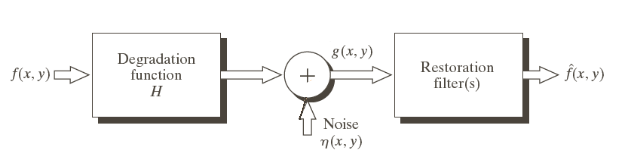
\includegraphics[width=.7\linewidth]{Picture/Restoration_Process}
\end{center}
In figura si vede un tipico processo di restoration: si parte dall'immagine originale ($f(x,y)$), perfetta, si passa attraverso un primo filtro che danneggia l'immagine (ad esempio la macchina non ha messo correttamente a fuoco), assumeremo che questo filtro sia lineare e spazio invariante. Durante il processo di acquisizione poi potrebbe essere sommato all'immagine del rumore (tipicamente pdovuto a imperfezioni del sensore) e si arriva all'immagine degradata ($g(x,y)$). All'immagine rovinata si possono applicare uno o più filtri di restoration per ottenere una stima dell'immagine originale ($\hat{f}(x,y)$).

Siccome Assumiamo che i filtri che rovinano l'immagine siano lineari e spazio invarianti possiamo scrivere 
\begin{gather}
	g(x,y) = h(x,y)*f(x,y) + \eta(x,y)\\
	G(u,v) = H(u,v)\cdot F(u,v) + N(u,v)
\end{gather}
Dove le lettere maiuscole indicano la trasformata di Fourier della funzione con la minuscola.

\section{Rumore}
È un danno all'immagine dovuto all'ambiente e alla tipologia di acquisizione dell'immagine. Possiamo studiarne le proprietà attraverso lo spettro in frequenza (ad esempio spettro piatto per il rumore bianco) e in generale assumiamo sia spazio invariante.

\subsection{Stimare il rumore}
Oltre al rumore bianco l'immagine può essere affetta da rumori distribuiti in molti modi. Per stimare i parametri del rumore si possono adottare diverse tecniche.
\subsubsection{Rumore spazio invariante} 
\begin{wrapfigure}[11]{r}{.3\linewidth}
	\vspace{-.8cm}
	\centering
	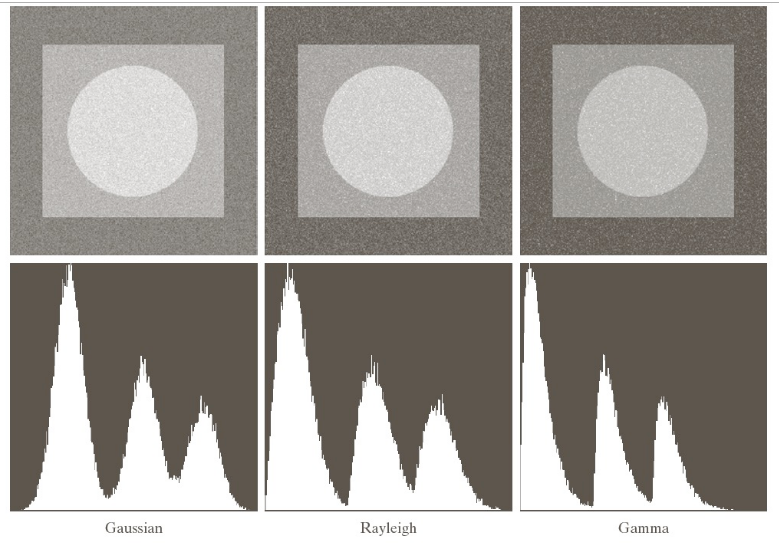
\includegraphics[width=.95\linewidth]{Picture/Noise_Distribution1}
	\\
	\vspace{.1cm}
	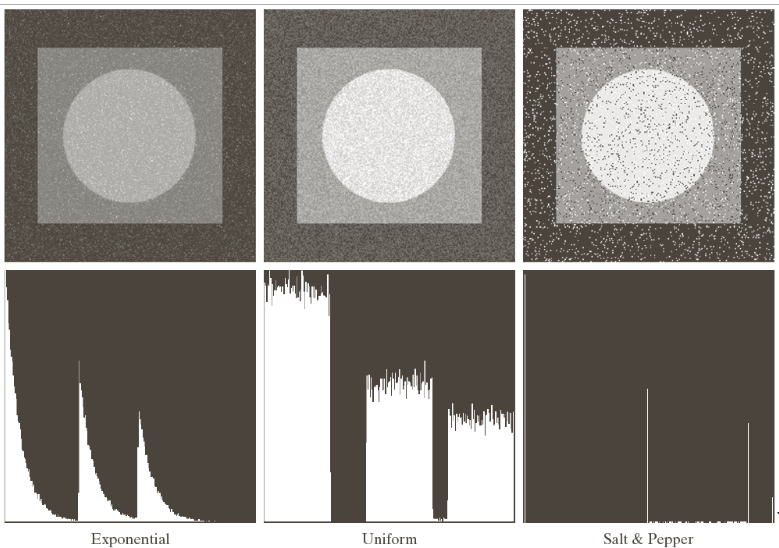
\includegraphics[width=.95\linewidth]{Picture/Noise_Distribution2}
\end{wrapfigure}
Siamo interessati a stimare la PDF del rumore, per fare questo si può considerare una zona dell'immagine che sappiamo avere uno stesso livello di grigio e studiare l'istogramma di quella zona, per osservare la distribuzione del rumore. Nelle immagini vediamo alcuni esempi di come differenti distribuzioni del rumore danneggiano immagini sintetizzate. Anche in questi esempi molto semplici è molto difficile capire il tipo di rumore senza guardare l'istogramma.

Capire la PDF del rumore è importante dato che sono stati ingegnerizzati  filtri apositi che, sfruttando le conoscenze a priori della PDF, correggono meglio i danni provocati da un certo tipo di rumore.

\subsubsection{Rumore spazio dipendente} 
\begin{wrapfigure}[9]{l}{.3\linewidth}
	\vspace{-.6cm}
	\centering
	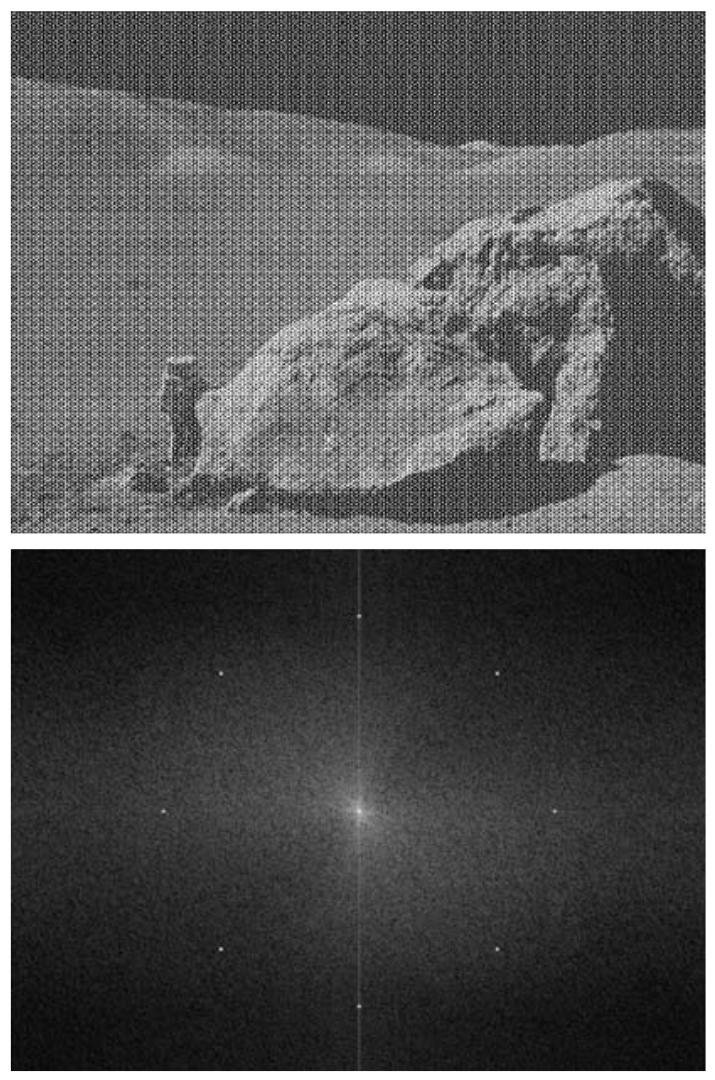
\includegraphics[width=.95\linewidth, height=4.5cm]{Picture/Periodic_Noise}
\end{wrapfigure}
Normalmente questo è dovuto al particolare processo di acquisizione, in questo caso ci concentriamo sul rumore periodico, che è un particolare tpo di rumore spazio dipendente. Il rumore periodico può essere individuato da dei picchi visibili nella trasformata di Fourier dell'immagine, è in questo domino che progettiamo i filtri per imuovere il rumore periodico. Ogni componente del rumore genera 2 picchi simmetrici nella trasformata.
\newpage

\section{Rumore spazio invariante}
Progettiamo dei \textbf{filtri nel dominio spaziale} per ridurre il rumore presente in un immagine. Questi filtri sono adatti quando nell'immagine è presente rumore additivo. Il modello di degradazione è:
\begin{gather}
	g(x,y) = f(x,y) + \eta(x,y)\\
	G(u,v) = F(u,v) + N(u,v)
\end{gather}
Nel prgettare questi filtri prenderemo in considerazione un pixel e i suoi vicini, questi possono essere disposti a croce, gli  8 tutti attorno oppure possiamo considerare un quadrato più grande, chiameremo $S_{xy}$ il vicinato (\textbf{neighbourhood}) del pixel a coordinate $(x,y)$
\subsection{Filtri semplici}
\subsubsection{Filtri che operano una media}
\begin{description}
	\item [Aritmetica] 
		\begin{equation}
			\hat{f} = \frac{1}{mn} \sum_{(s,t)\in S_{xy}} g(s,t)
		\end{equation}
		Il rumore è ridotto grazie al blurring, è l'unico filtro lineare (solo per questo ha senso studiare la risposta in frequenza);
	\item[Geometrica]
		\begin{equation}
			\hat{f} =\Bigg[\prod_{(s,t)\in S_{xy}} g(s,t)\Bigg]^{\frac{1}{mn}}
		\end{equation}
		Riduce il rumore ma preserva più dettagli rispetto alla media aritmetica;
	\item[Armonica]
		\begin{equation}
			\hat{f} = \frac{mn} {\sum_{(s,t)\in S_{xy}} \frac{1}{g(s,t)}}
		\end{equation}
		Adatta a ridurre il rumore gaussiano e di tipo sale, fallisce con il rumore pepe;
	\item[Contrarmonica]
		\begin{equation}
			\hat{f} = \frac{\sum_{(s,t)\in S_{xy}} g(s,t)^{Q+1}} {\sum_{(s,t)\in S_{xy}} g(s,t)^Q}
		\end{equation}
		$Q$ è l'ordine della media, se $Q>0$ adatta per rumore pepe, se $Q<0$ adatta per rumore sale, se $Q=0$ o $Q=-1$ si riade in media aritmetica o armonica rispettivamente.
\end{description}

\subsubsection{Filtri basati sull'ordinamento dei livelli d'intensità}
Questi filtri sono adatti alla rimozione degli outlier.
\begin{description}
	\item[Mediana]
		\begin{equation}
			\hat{f} = \underset{(s,t)\in S_{xy}}{\text{median}}\ g(s,t)
		\end{equation}
		Adatto a rimuovere rumore impulsivo, può rovinare i bori sottili;
		\item[Max/Min]
		\begin{equation}
			\hat{f} = \underset{(s,t)\in S_{xy}}{\text{max/min}}\ g(s,t)
		\end{equation}
		Adatti a rimuovere rispettivamente rumore pepe e sale;
		\item[Punto medio]
		\begin{equation}
			\hat{f} = \frac{\underset{(s,t)\in S_{xy}}{\text{max}}\ g(s,t) + \underset{(s,t)\in S_{xy}}{\text{min}}\ g(s,t)}{2}
		\end{equation}
		Adatto a rimuovere rumore casuale gaussiano o uniforme;
		\item[Alfa trimmed]
		\begin{equation}
			\hat{f} = \frac{1}{mn - d} \sum_{(s,t)\in S_{xy}} g'(s,t)
		\end{equation}
		Prima di calcolare la media vengono scartati i $d/2$ valori più piccoli e i $d/2$ valori più grandi. È adatto per rimuovere rumore sale e pepe e gaussiano assieme.
\end{description}

\subsection{Filtri adattativi}
Sono filtri che adattano il loro comportamento in base alle caratteristiche locali dell'immagine, tipicamente si considera una finestra $m\times n$ che rappresenta il vicinato di un pixel e si confrontano le caratteristiche della finestra con quelle dell'immagine intera per dosare il comportamento del filtro.
\subsubsection{Media adattativa}
	\begin{equation}
		\hat{f}(x,y) = g(x,y) - \frac{\sigma_{\eta}^2}{\sigma_L^2}[g(x,y) - m_L]
	\end{equation}
Dove $\sigma_{\eta}$ è la varianza del rumore, $\sigma_L$ è la varianza locale e $m_L$ è la media locale. La media locale rappresenta la luminanza nella zona che stiamo considerando, mentre la varianza locale il contrasto. 
\newpage
A seconda del rapporto tra la varianza del rumore e la varianza locale il filtro si comporta in modo diverso:
\begin{itemize}
	\item $\sigma_{\eta} = 0$ non c'è rumore quindi $\hat{f}(x,y) = g(x,y) = f(x,y)$;
	\item $\sigma_L \gg \sigma_{\eta}$ molto contrasto, ci sono dei bordi, quindi non bisogna filtrare troppo per non rovinare i gettagli $\hat{f}(x,y) \approx g(x,y)$;
	\item $\sigma_L = \sigma_{\eta}$ la finestra ha le stesse caratteristiche dell'immagine, il filtro si comporta esattamente come la media;
	\item $\sigma_{\eta} > \sigma_L$ si forza $\sigma_{\eta} = \sigma_L$ per non ottenere dei valori negativi, questo potrebbe rendere necessario riscalare i valori dell'immagine per non perdere della dinamica dell'immagine.
\end{itemize}

Affinché questo filtro possa funzionare correttamente è essenziale avere una stima accurata della varianza del rumore.

\subsubsection{Mediana adattativa}
Questo filtro ha lo scopo di preservare i bordi, rimuovere il rumore impulsivo, fare smoothing del rumore random senza allargare o assottigliare i bordi.
\vspace{.5cm}

\begin{algorithmic}
	\Function{AdaptativeMedian}{ }
		\State $S_{xy} \gets S_{min}$
		\While{$S_{xy} \leq S_{max}$}
			\State $A_1 \gets z_{med} - z_{min}$
			\State $A_2 \gets z_{med} - z_{max}$
			\If{$A_1 > 0 \textbf{ and } A_2 < 0$}
				\State $B1 \gets z_{xy} - z_{min}$
				\State $B1 \gets z_{xy} - z_{max}$
				\If{$B_1 > 0 \textbf{ and } B_2 < 0$}
					\State \Return $z_{xy}$
				\Else
					\State \Return $z_{med}$
				\EndIf
			\Else
				\State $S_{xy} \gets$ \Call{IncrementNeighbourhood}{ }
			\EndIf
		\EndWhile
		\State \Return $z_{med}$
	\EndFunction    
\end{algorithmic}

Dove:
\begin{itemize}
	\item $S_{xy}$: Area del vicinato del pixel $(x,y)$;
	\item $z_{min}$: Intensità minima nell'area considerata;
	\item $z_{max}$: Intensità massima nell'area considerata;
	\item $z_{med}$: Intensità media nell'area considerata;
	\item $z_{xy}$: Intensità del pixel $(x,y)$;
	\item $S_{min}$:Area di partenza del vicinato;
	\item $S_{max}$: Massima area del vicinato consentita.
\end{itemize}

Come si vede questo filtro è in grado di modificare, entro certi limiti, la dimensione della finestra di vicinato. Il filtro calcola la mediana, se questa corrisponde al minimo o al massimo dell'intensità si aumenta la dimensione della finestra, altrimenti si decide se restituire la mediana o il valore del pixel. Si restituisce il valore del pixel se questo ha le stesse caratteristiche che abbiamo richiesto per la mediana (non è né un minimo né un massimo di intensità).

\section{Rumore spazio dipendente}
Progettiamo dei filtri \textbf{nel dominio della frequenza} per ridurre il rumore additivo spazio dipendente.
Per descrivere il rumore osserveremo quali sono le sue componenti nella trasformata di Fourier e cereremo di isolare l'immagine rispetto al rumore.

\subsection{Notch Filter}
Il rumore periodico si individua facendo la trasformata e cercando dei picchi nella stessa. Ogni componente genera 2 picchi simmetrici rispetto all'origine. Per rimuovere il rumore periodico si può usare un filtro \textbf{notch} $H_{NR}$. Questo è costituito dal prodotto di filtri passa alto centrati sui picchi di rumore.
\begin{equation}
	H_{NR}(u,v) = \prod_{k=1}^{Q} H_k(u,v) H_{-k}(u,v)
\end{equation}
Dove $ H_k(u,v)$ è il filtro passa alto centrato in $u_k,v_k$ e $H_{-k}(u,v)$ è il simmetrico rispetto all'origine.

Ciascun $H_k$ può essere costruito utilizzando diverse forme (ideale, gaussiano, butterworth, ecc\dots) indipendentemente dagli altri filtri passa alto, l'importante è che $H_{k}(u,v)$ e $H_{-k}(u,v)$ abbiano la stessa forma.

\begin{wrapfigure}{r}{.5\linewidth}
	\vspace{-.4cm}
	\centering
	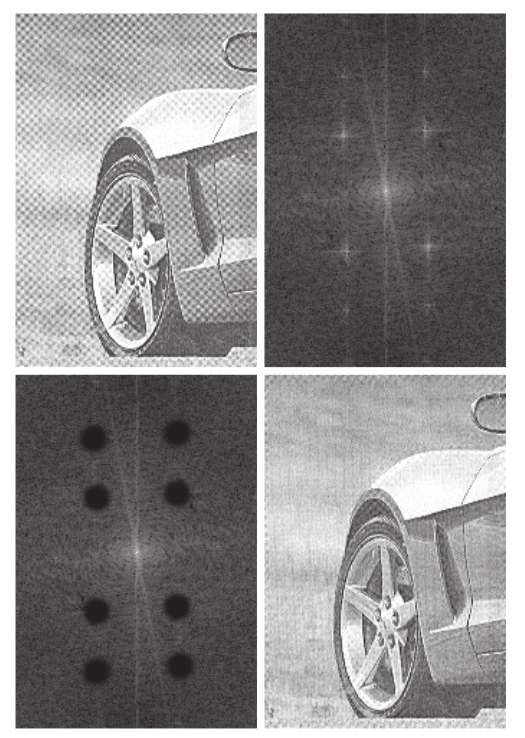
\includegraphics[width=.95\linewidth]{Picture/Notch}
\end{wrapfigure}
Per fare image enanchement è sufficiente centrare i filtri passa alto nei picchi di rumore visibili nella trasformata di Fourier e filtrare l'immagine utilizzando il filtro notch ottenuto componendo i passa alto. Il risultato che si ottiene è spesso più soddisfacente rispetto all'immagine che si otterrebbe con dei filtri di blurring. Inoltre se i picchi di rumore sono sufficientemente distanti dalle frequenze che caratterizzano l'immagine il filtro notch non rovina i dettagli, neppure quelli più fini. L'immagine mostra la situazione originale e l'applicazione dei filtri passa alto in corrispondenza dei picchi di rumore, come si vede il risultato è soddisfacente.

\subsubsection{Optimum Notch}
Costruiamo a partire dal filtro notch un filtro adattativo che pesi l'effetto del filtro notch a seconda delle caratteristiche locali dell'immagine. Come sempre consideriamo il vicinato $S_{xy}$ del pixel $(x,y)$ e ricaviamo un filtro che minimizzi la varianza locale dell'immagine ricostruita $\hat{f}(x,y)$. Per costruire l'optimum notch abbiamo bisogno di:
\begin{itemize}
	\item filtro che isoli il rumore: $H_{NP} = 1 - H_{NR}$
	\item rumore stimato: $\eta(x,y)= \mathfrak{F}^{-1}\{N(u,v)\}= \mathfrak{F}^{-1}\{H_{NP}(u,v)G(u,v)\}$
	\item immagine ricostruita: $\hat{f} = g(x,y) - w(x,y)\eta(x,y)$
\end{itemize}
Dove pesiamo il rumore con $w(x,y)$ perché non è il rumore esatto, ma solo una stima.

Siamo pronti per calcolare la varianza locale dell'immagine ricostruita; chiamiamo il valor medio di una misura come la misura stessa con una barretta sopra, ad esempio $\overline{\eta}$ è il valor medio del rumore nella finestra considerata.
\begin{align}
	&\sigma^2(x,y) = \frac{1}{mn} \sum_{(r,c)\in S_{xy}}\Big[\hat{f}(r,c) - \overline{\hat{f}}\Big] =	& \\
	&= \frac{1}{mn} \sum_{(r,c)\in S_{xy}} \Big\{ [g(c,r) -w(c,r)\eta(c,r)] - [\overline{g} -\overline{w\eta}]\Big\}^2 = & \text{def. di } \hat{f}  \notag \\
	&= \frac{1}{mn} \sum_{(r,c)\in S_{xy}} \Big\{ [g(c,r) -w(c,r)\eta(c,r)] - [\overline{g} - w(x,y)\overline{\eta}]\Big\}^2 & \qquad\overline{w}= w(x,y)  \notag
\end{align}
Nell'ultimo passaggio approssimo i pesi della finestra al peso del pixel centrale ($w(c,r) = w(x,y)$), quindi la media sarà il peso del pixel centrale. 

Possiamo derivare la varianza in funzione di $w(x,y)$ e imporla a $0$, si ottiene il vincolo su $w(x,y)$:
\begin{equation}
	w(x,y) = \frac{\overline{g\cdot\eta} - \overline{g}\cdot\overline{\eta}}{\overline{\eta^2} - \overline{\eta}^2}
\end{equation}

\section{Danni lineari spazio invarianti}
Le immagini che prendiamo in considerazione ora sono affette da una degradazione lineare spazio invariante, cioè l'immagine è stata trasformata da un filtro lineare spazio invariante. Questo significa che possiamo modellare l'immagine acquisita come:
\begin{gather}
	g(x,y) = h(x,y)*f(x,y)\\
	G(u,v) = H(u,v)\cdot F(u,v)
\end{gather}
Per ripristinare l'immagine quindi è necessario operare una deconvoluzione nel dominio spaziale o una semplice divisione nel dominio della frequenza, data la semplicità si sceglie sempre il secondo. La deconvoluzione di filtri non lineari o spazio dipendenti è molto più complessa o, in certi casi, addirittura irrisolvibile.

\subsection{Filtro inverso}
L'idea più semplice per recuperare un immagine danneggiata da un filtro lineare spazio invariante è quella di costruire il filtro inverso. Il filtro inverso, se esiste ed è stabile permette di ricostruire l'immagine di partenza. Vediamo ora alcuni metodi per risalire al filtro che ha danneggiato l'immagine e quindi per poter stimare il filtro inverso.

\subsubsection{Stima per osservazione}
Per stimare il filtro che ha rovinato l'immagine $g(x,y)$ possiamo isolare una piccola area $g_s(x,y)$ dell'immagine che sia facile da ricostruire, ripararla empiricamente (anche con un semplice programma di fotoritocco) in modo da ottenere $\hat{f}_s(x,y)$; ora possiamo ottenere il filtro che ha degradato la piccola area come:
\begin{equation}
	H_s(u,v) = \frac{G_s(u,v)}{\hat{F}_s(u,v)}
\end{equation}
Possiamo poi costruire il filtro $H(u,v)$ a partire da $H_s(u,v)$ per scalamento.

\subsubsection{Stima sperimentale}
Dato che stiamo considerando filtri lineari spazio invarianti questi possono essere caratterizzati dalla risposta all'impulso. Per studiare la risposta all'impulso del sistema ottico acquisisco un singolo punto luminoso (molto intenso per evitare il rumore) nelle stesse condizioni in cui ho acquisito l'immagine che voglio recuperare. Dato che la DFT dell'impulso è nota ed è una costante $A$ ricavare il filtro è molto semplice:
\begin{equation}
	H(u,v) = \frac{G(u,v)}{A}
\end{equation}

\subsubsection{Stima con modello}
Esistono diversi modelli che descrivono alcuni fenomeni fisici comuni, come la turbolenza atmosferica, la presenza di nebbia o foschia, ecc\dots oppure delle imprecisioni durante l'acquisizione dell'immagine come il movimento della camera. Se si ha a disposizione il modello di degradazione per progettare il filtro che ha rovinato l'immagine è sufficiente impostare correttamente i parametri del modello per ricostruire filtro e filtro inverso.

\subsubsection{Problemi del filtro inverso}
Questo approccio funziona se l'immagine acquisita $G(u,v)$ non è affetta da altri tipi di rumore, infatti in generale l'immagine che otteniamo dopo il ripristino sarà data da:
\begin{equation}
	\hat{F}(u,v) = \frac{G(u,v)}{H(u,v)} = F(u,v) + \frac{N(u,v)}{H(u,v)}
\end{equation}
\begin{wrapfigure}{r}{.5\linewidth}
	\centering
	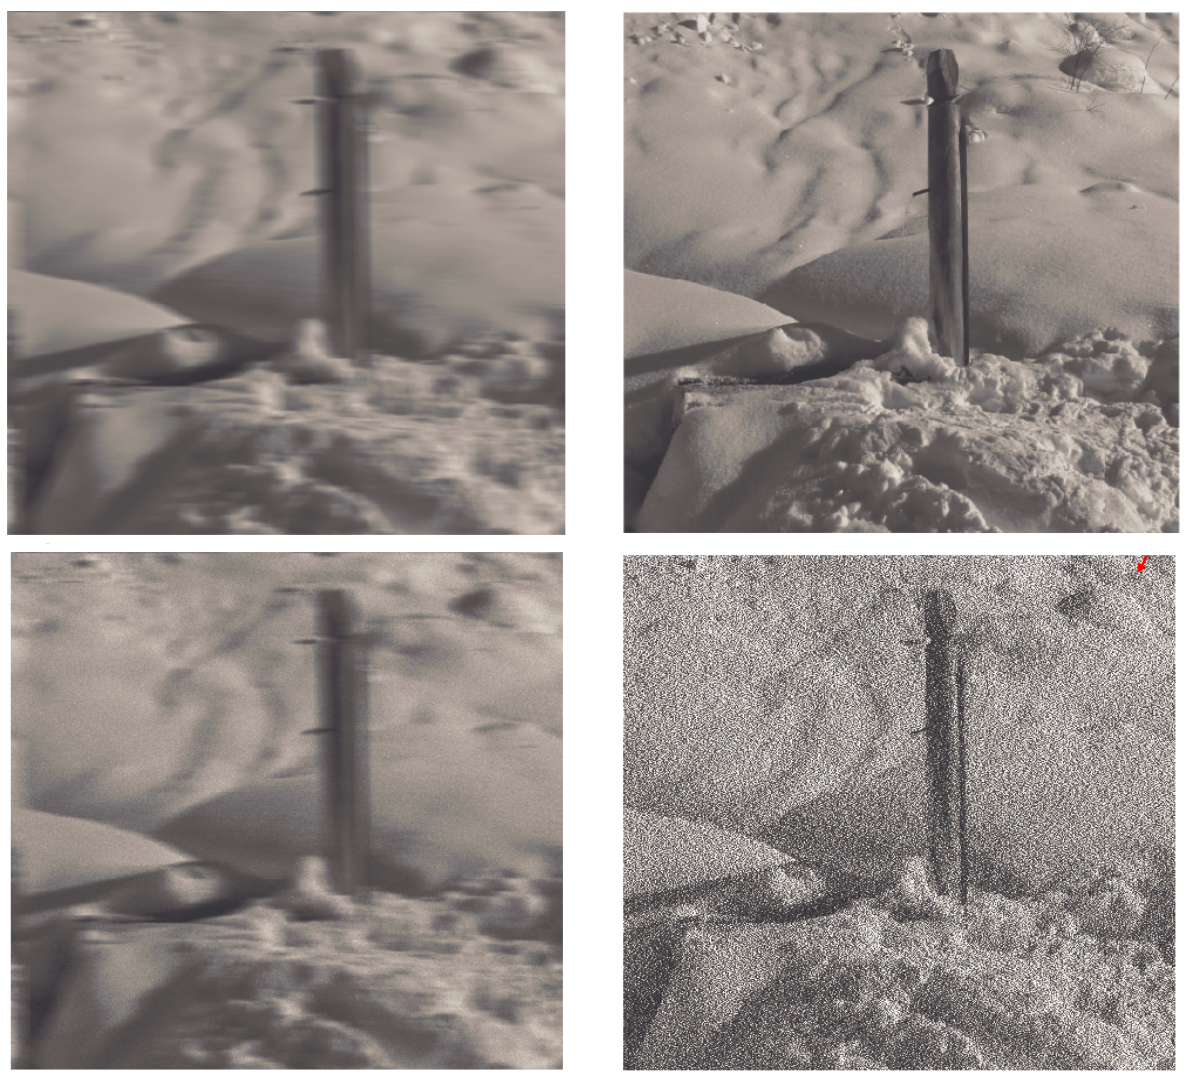
\includegraphics[width=.95\linewidth]{Picture/Inverse_Filter}
\end{wrapfigure}
Dove la frazione indica la deconvoluzione tra il rumore e il filtro che abbiamo usato per ripristinare l'immagine. Dei valori prossimi a zero nel filtro possono aumentare molto la componente rumorosa e l'immagine che si ottiene risulta essere fortemente rovinata, nella figura si vede un esempio di immagine ricostruita con il filtro inverso che è stato modellato seguendo il movimento della camera. La prima coppia di immagini non è affetta da rumore, mentre la seconda sì e anche se nell'immagine mossa il rumore si nota poco in quella ricostruita predomina sull'immagine.

\subsection{Wiener filter}
Il problema del filtro inverso è stato studiatissimo e sono state proposte molte soluzioni che riducessero gli effetti mostrati sopra. Il filtro di Wiener migliora le prestazioni del filtro inverso minimizzando lo scarto quadratico medio (MSE Mean Square Error). Vogliamo minimizzare
\begin{equation}
	E\Big\{(f-\hat{f})^2\Big\}
\end{equation}
Se assumiamo oltre al filtro lineare spazio invariante che il rumore sia decorrelato dall'immagine e che almeno uno tra immagine e rumore abbia media nulla si può ricavare che il minimo del MSE è dato da un'immagine ricostruita con questa forma:
\begin{equation}
	\hat{F}(u,v) = \Bigg[\frac{H^*(u,v)}{|H(u,v)|^2 + S_{\eta}(u,v) / S_f(u,v)}\Bigg]G(u,v)
\end{equation}
Dove:
\begin{itemize}
	\item $H(u,v)$: filtro che ha danneggiato l'immagine
	\item $H^*(u,v)$: complesso coniugato di $H(u,v)$
	\item $|H(u,v)|^2 = H^*(u,v) H(u,v)$
	\item $S_{\eta}(u,v) = |N(u,v)|^2$: spettro di potenza del rumore
	\item $S_f(u,v) = |F(u,v)|^2$: spettro di potenza dell'immagine originale
\end{itemize}
\newpage
Al denominatore vediamo l'inverso del rapporto segnale rumore, infatti $S_{\eta}(u,v) / S_f(u,v) = 1/SNR$. Questo ci dice che il filtro di Wiener diventa il filtro inverso se a una data frequenza il rapporto segnale rumore tende a infinito, mentre cancella le frequenze dominate dal rumore.

È possibile semplificare questo filtro assumendo che il rumore sia bianco, quindi $S_{\eta}(u,v) / S_f(u,v) \rightarrow \sigma^2/ S_f(u,v)$, inoltre dato che in generale lo spettro dell'immagine originale non è noto assumiamo che il rapporto segnale rumore sia costante e lo consideriamo un parametro $K$ del filtro. Il filtro di Wiener diventa quindi:
\begin{equation}
	H(u,v) = \frac{H^*(u,v)}{|H(u,v)|^2 +K} = \frac{1}{H(u,v)}\frac{|H(u,v)|^2}{|H(u,v)|^2 +K} 
\end{equation}

\subsection{CLSF}
Il filtro di Wiener necessita dello spettro dell'immagine e del rumore, o almeno di una loro stima, dato che queste informazioni non sempre sono disponibili sono stati sviluppati altri filtri, come il Constrained Least Squares Filter. Questo filtro parte dall'idea che il filtro inverso fallisce perché il rumore che ha solitamente spettro piatto viene aumentato moltissimo specie alle alte frequenze dove il filtro ha valori molto bassi (ricordiamo che il filtro si trova a denominatore). Per impedire questo effetto si cerca un risultato più smooth minimizzando il laplaciano:

\begin{equation}
	\sum_{x=0}^{M}\sum_{y=0}^{N} \big[\nabla^2f(x,y)\big]
\end{equation}
La soluzione che minimizza il laplaciano è:
\begin{equation}
	\hat{F}(u,v) = \Bigg[\frac{H^*(u,v)}{|H(u,v)|^2 + \gamma|P(u,v)|^2}\Bigg]G(u,v)
\end{equation}
Dove:
\begin{itemize}
	\item $P(u,v)$ è la trasformata dell'operatore laplaciano: $P(u,v) = \mathfrak{F} \Big( \Big[
	\begin{smallmatrix}
		0&-1&0\\
		-1&4&-1\\
		0&-1&0
	\end{smallmatrix} \Big]\Big)$ 
	\item $\gamma$ è un parametro da settare per fare in modo che il filtro riesca effettivamente a isolare il rumore. Siccome $\gamma$ è proprio il parametro più delicato da stimare questo può essere ottenuto \textbf{iterativamente}.
\end{itemize}

\subsection{Filtro con media geometrica}
È possibile generalizzare il filtro di Wiener in uno che ricordi la media geometrica. Questo filtro è molto utile dato che controllando i suoi 2 parametri si possono implementare filtri molto diversi utili in tanti ambiti. Il filtro generale genera un'immagine ricostruita in questo modo:
\begin{equation}
	\hat{F}(u,v) = \left[\frac{H^*(u,v)}{|H(u,v)|^2}\right]^{\alpha}\left[\frac{H^*(u,v)}{|H(u,v)|^2 +\beta\left[\frac{S_{\eta}(u,v)}{S_f(u,v)}\right]}\right]^{1-\alpha}G(u,v)
\end{equation}
Dove $\alpha \geq 0$ e $\beta \geq 0$ sono i parametri e a seconda del loro valore si hanno diversi comportamenti:
\begin{itemize}
	\item $\alpha = 1$: filtro inverso;
	\item $\alpha = 0$: filtro di Wiener parametrico ($\beta$ = 1 Wiener standard);
	\item $\alpha = \frac{1}{2}$: si calcola la media geometrica delle quantità tra parentesi
	\item $\alpha = \frac{1}{2}$ e $\beta = 1$: filtro equalizzatore dello spettro;
	\item $\alpha<\frac{1}{2}$: il filtro si comporta più come Wiener;
	\item $\alpha>\frac{1}{2}$: il filtro si comporta più come filtro inverso.
\end{itemize}
\subsection{Esempi}
\begin{wrapfigure}{r}{.5\linewidth}
	\vspace{-.8cm}
	\centering
	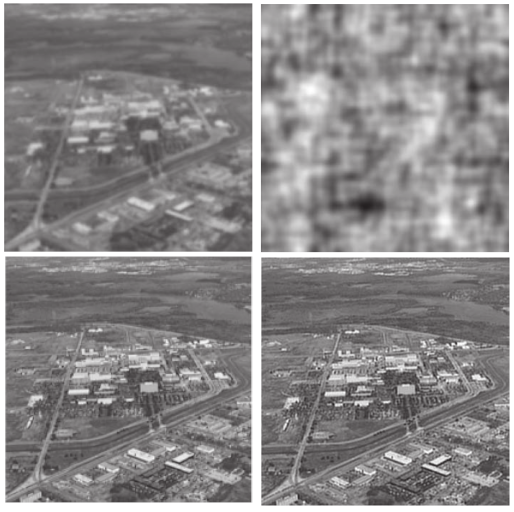
\includegraphics[width=.95\linewidth]{Picture/Filter_Example}
\end{wrapfigure}
Le immagini sono disposte $\left(
\begin{smallmatrix}
	1&2\\
	3&4 
\end{smallmatrix}
\right)
$ e mostrano l'applicazione di diversi filtri a un'immagine rovinata da turbolenza atmosferica e affetta da rumore additivo:
\begin{enumerate}
	\item Immagine originale;
	\item Filtro inverso;
	\item Filtro Wiener;
	\item Filtro CLSF.
\end{enumerate}
